\maketitle

% Abstract section
\begin{minipage}[t]{\textwidth}
	
	% chapters/00_abstract.tex
	\begin{abstract}
		انگیزه‌ای از موفقیت گسترده شبکه‌های عمیق کانولوشنی، علاقه زیادی برای تعمیم کانولوشن‌ها به منیفلدهای غیراقلیدسی وجود دارد.
		یک پیچیدگی عمده در مقایسه با فضاهای مسطح این است که مشخص نیست کرنل کانولوشن باید در کدام تراز روی یک منیفلولد اعمال شود.
		دلیل اساسی این ابهام آن است که منیفلولدهای عمومی دارای انتخاب متعارف چارچوب‌های مرجع (گیج) نیستند.
		بنابراین کرنل‌ها و ویژگی‌ها باید نسبت به \emph{مختصات دلخواه} بیان شوند.
		ما استدلال می‌کنیم که انتخاب خاص مختصات‌بندی نباید بر استنتاج شبکه تأثیر بگذارد -- آن باید \emph{مستقل از مختصات} باشد.
		تقاضای همزمان برای استقلال مختصات و اشتراک وزن منجر به الزامی روی شبکه می‌شود تا تحت تبدیل‌های گیج محلی (تغییرات چارچوب‌های مرجع محلی) \emph{تناوب‌پذیر} باشد.
		ابهام چارچوب‌های مرجع بدین‌گونه به $G$-\emph{ساختار} منیفلولد بستگی دارد،
		به طوری که سطح لازم تناوب‌پذیری گیج توسط \emph{گروه ساختار}~$G$ متناظر تجویز می‌شود.
		کانولوشن‌های مستقل از مختصات ثابت می‌شوند که نسبت به آن \emph{ایزومتری‌هایی} که تقارن‌های $G$-ساختار هستند تناوب‌پذیر باشند.
		نظریه حاصل به شکل آزاد از مختصات بر حسب بندل‌های فیبر فرمول‌بندی می‌شود.
		برای نمونه‌سازی طراحی کانولوشن‌های مستقل از مختصات، ما شبکه کانولوشنی روی نوار موبیوس پیاده‌سازی می‌کنیم.
		عمومیت فرمول‌بندی هندسه دیفرانسیل ما از شبکه‌های کانولوشنی با بررسی گسترده ادبیات نشان داده می‌شود
		که تعداد زیادی از شبکه‌های کانولوشنی اقلیدسی، شبکه‌های کانولوشنی کروی و شبکه‌های کانولوشنی روی سطوح عمومی را به عنوان نمونه‌های خاص کانولوشن‌های مستقل از مختصات توضیح می‌دهد.
		
		\begin{figure}[H]
			\centering
			\vspace*{2.5ex}
			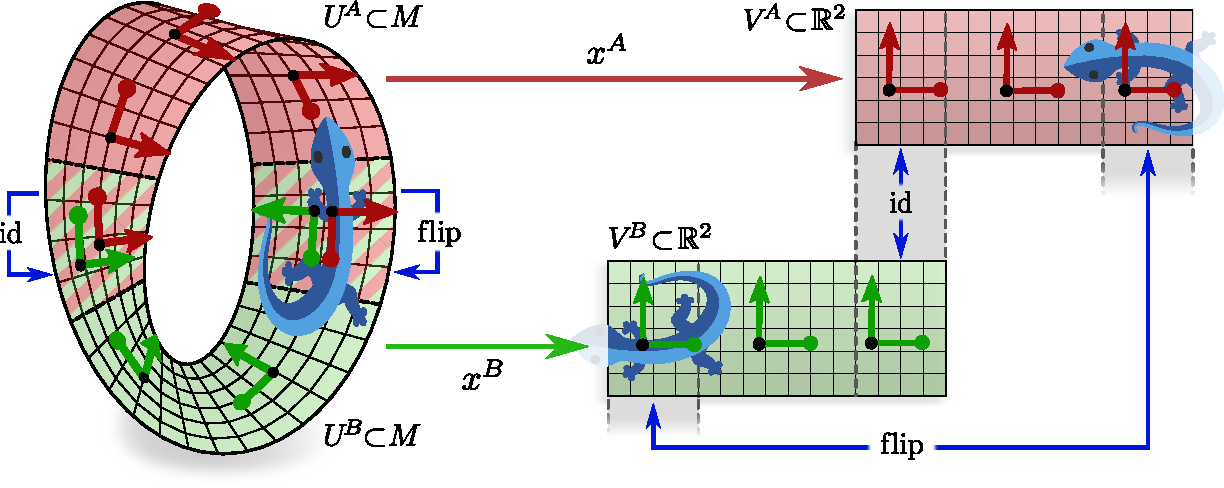
\includegraphics[width=.94\columnwidth]{figures/mobius_conv_gauges.pdf}
			\caption{نمایش کانولوشن روی نوار موبیوس با گیج‌های مختلف}
		\end{figure}
	\end{abstract}
	
	% hack to keep abstract on front page, even though it overflows
	\vspace*{-20ex}
	
\end{minipage}